\subsection{Design of experiments}
%When comparing images taken of the same scene, three common changes are scale, rotation and illumination. Because of this, I have designed my experiments to evaluate image descriptors on a roughly equal amount of images mainly varying in scale, rotation and illumination. 
For this assignment a subset of the 'HPatches' data set has been chosen, namely the first 10 series with illumination changes and the 10 fist series with view point changes. Three image descriptors, namely SIFT, ORB and SURF \todo{CHANGE} will then be evaluated on the aforementioned data. A consideration for the experiments have been, that an image descriptor both chooses a location in an image which it finds fitting, and it describes this location. That is, we both get key points and descriptors for each found feature in the image. To evaluate the key points we use \textit{mean localization error}, to evaluate descriptors we use \textit{nearest neighbour mean average precision}, and to evaluate the image descriptor as a whole, we use \textit{homography estimation}. Before going into details with these error measures, we will first look at how we classify true positives, false positives and false negative detections.\\
For each pair of images considered, we apply the image descriptor to both images, and the detections made in \textit{image 1} are considered ground truth whereas the detections made in \textit{image 2} are considered candidate points. If there is a perspective change between the two images, the ground truths are warped into the perspective of the candidate points. To detect false positives, we go through each detection in our candidate points, and each candidate point which does not have a similar ground truth is considered a false positive. To detect false negatives we go through each ground truth and if it does not have a similar candidate point it is a false negative. A true positive can be measured as either each candidate point which has a similar ground truth, or each ground truth which has a similar candidate point. This 'similar' / $\epsilon$ term is measured as the L2 norm, and can be increased / shrunk in order to create precision / recall curves. We will compute precision and recall by starting with $\epsilon = 0$ and increase it.
As we might have more ground truths than candidate points and vice versa, the recall and precision is rescaled to always go from 0 to 1. 
To ensure correct curves, 1 - recall will be used to compute precision / recall curves. An example of a precision / recall curve can be seen in \autoref{PRCurve}. Each ground truth or candidate point can only be matched once, that is, if we have two candidate points around a ground truth, only one of them will be considered a true positive whereas the other will be considered a false positive.

\begin{figure}[h]
	\centering
	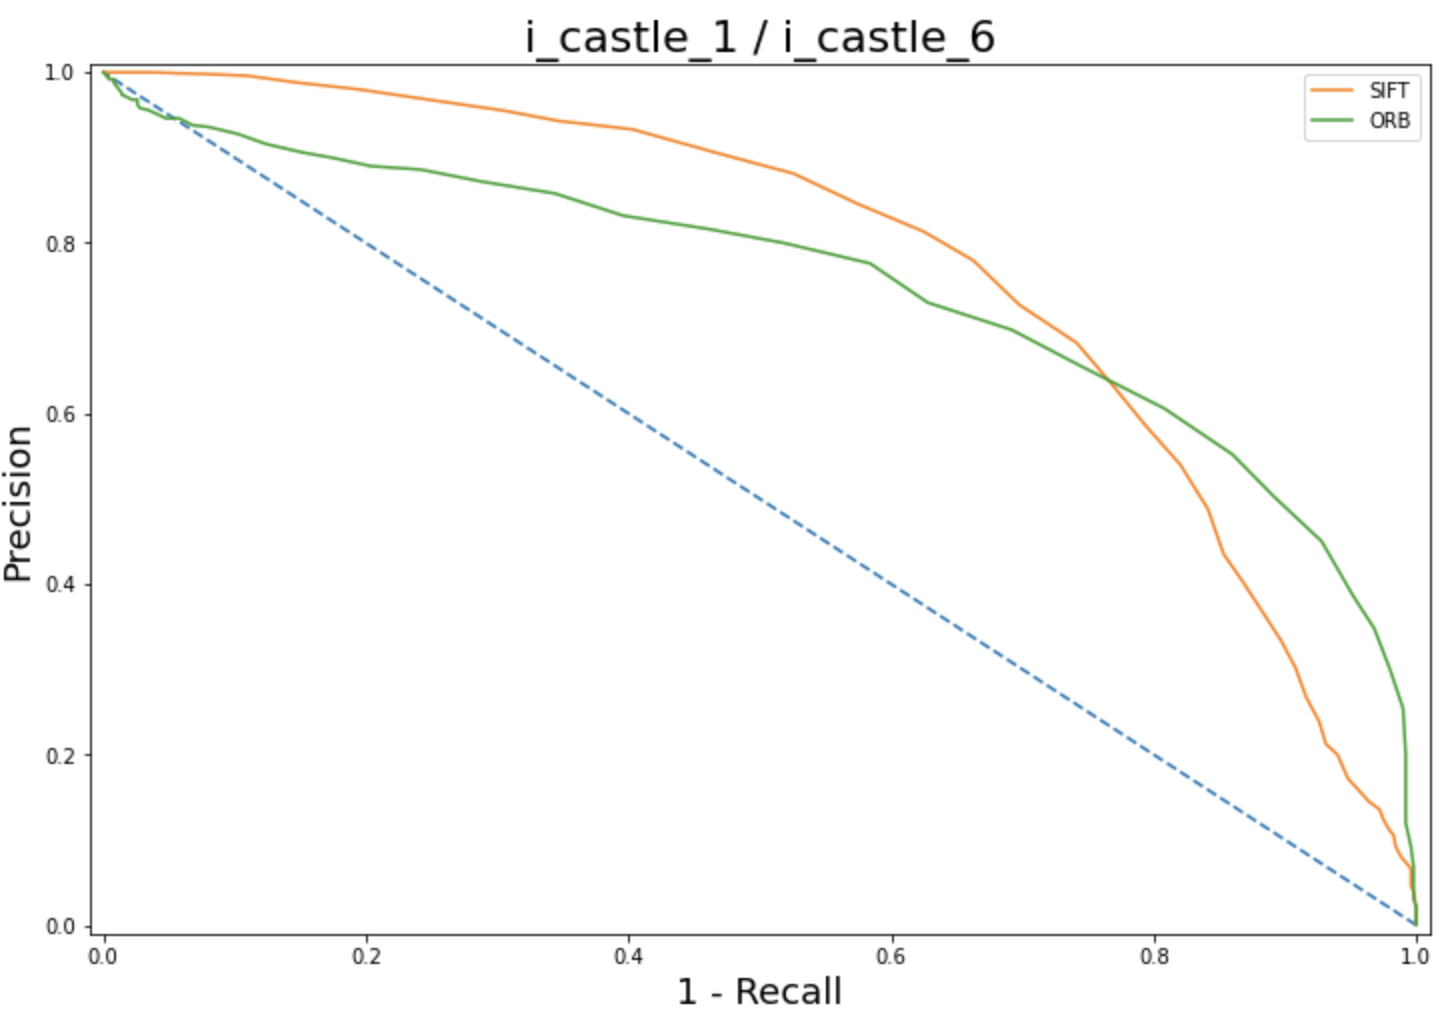
\includegraphics[width=0.68\linewidth]{Materials/PRCurve}
	\caption{Precision / recall curve for two images in the castle series.}
	\label{PRCurve}
\end{figure}